\documentclass[tikz,border=2pt]{standalone}
\usepackage{amsmath}
\usepackage{stix2}
\usepackage{bm}
\usetikzlibrary{arrows.meta}

\begin{document}
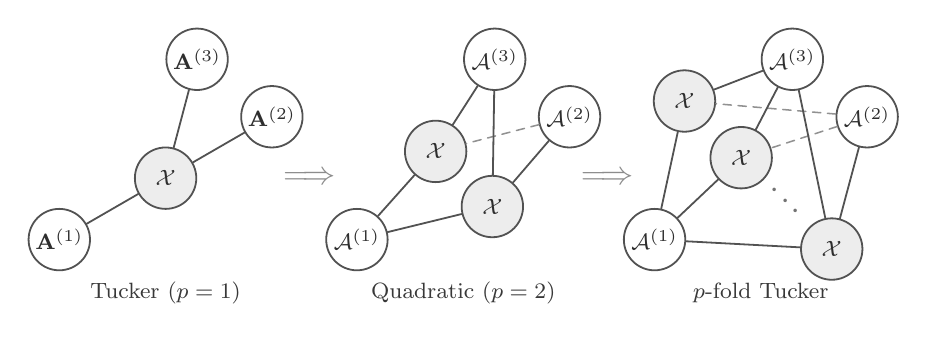
\begin{tikzpicture}[
  line cap=round,
  line join=round,
  >=Latex,
  font=\footnotesize,
  factor/.style={
    circle,
    draw=black!68,
    fill=white,
    minimum size=7.8mm,
    inner sep=0pt,
    line width=0.65pt,
    text=black!82
  },
  core/.style={
    circle,
    draw=black!68,
    fill=black!7,
    minimum size=7.8mm,
    inner sep=0pt,
    line width=0.65pt,
    text=black!82
  },
  edge/.style={draw=black!68,line width=0.65pt},
  hedge/.style={
    draw=black!43,
    dashed,
    line width=0.55pt,
    dash pattern=on 3.0pt off 2.4pt
  },
  arrow/.style={text=black!45,font=\large},
  captionlabel/.style={font=\footnotesize,text=black!78}
]

% Tucker: one core connected to the three mode factors.
\begin{scope}[xshift=0cm]
  \node[factor] (f1) at (0.00,0.00) {$\mathbf A^{(1)}$};
  \node[factor] (f2) at (2.70,1.56) {$\mathbf A^{(2)}$};
  \node[factor] (f3) at (1.75,2.29) {$\mathbf A^{(3)}$};
  \node[core]   (c1) at (1.35,0.78) {$\mathcal X$};

  \draw[edge] (f1) -- (c1);
  \draw[edge] (f2) -- (c1);
  \draw[edge] (f3) -- (c1);

  \node[captionlabel] at (1.35,-0.68) {Tucker $(p=1)$};
\end{scope}

\node[arrow] at (3.18,0.78) {$\Longrightarrow$};

% Quadratic term: two copies of the core share the three mode maps.
\begin{scope}[xshift=3.78cm]
  \node[factor] (f1) at (0.00,0.00) {$\mathcal A^{(1)}$};
  \node[factor] (f2) at (2.70,1.56) {$\mathcal A^{(2)}$};
  \node[factor] (f3) at (1.75,2.29) {$\mathcal A^{(3)}$};
  \node[core] (c1) at (1.00,1.12) {$\mathcal X$};
  \node[core] (c2) at (1.72,0.42) {$\mathcal X$};

  \draw[edge]  (f1) -- (c1);
  \draw[edge]  (f1) -- (c2);
  \draw[hedge] (f2) -- (c1);
  \draw[edge]  (f2) -- (c2);
  \draw[edge]  (f3) -- (c1);
  \draw[edge]  (f3) -- (c2);

  \node[captionlabel] at (1.35,-0.68) {Quadratic $(p=2)$};
\end{scope}

\node[arrow] at (6.96,0.78) {$\Longrightarrow$};

% General p-fold term: the omitted copies follow the same connections.
\begin{scope}[xshift=7.56cm]
  \node[factor] (f1) at (0.00,0.00) {$\mathcal A^{(1)}$};
  \node[factor] (f2) at (2.70,1.56) {$\mathcal A^{(2)}$};
  \node[factor] (f3) at (1.75,2.29) {$\mathcal A^{(3)}$};
  \node[core] (c1) at (1.10,1.04) {$\mathcal X$};
  \node[core] (c2) at (0.38,1.76) {$\mathcal X$};
  \node[core] (cp) at (2.25,-0.12) {$\mathcal X$};

  \draw[edge]  (f1) -- (c1);
  \draw[edge]  (f1) -- (c2);
  \draw[edge]  (f1) -- (cp);
  \draw[hedge] (f2) -- (c1);
  \draw[hedge] (f2) -- (c2);
  \draw[edge]  (f2) -- (cp);
  \draw[edge]  (f3) -- (c1);
  \draw[edge]  (f3) -- (c2);
  \draw[edge]  (f3) -- (cp);

  \node[font=\large,rotate=-45,text=black!55] at (1.68,0.46) {$\cdots$};
  \node[captionlabel] at (1.35,-0.68) {$p$-fold Tucker};
\end{scope}

\end{tikzpicture}
\end{document}
